\documentclass[conference,a4paper]{IEEEtran}
\usepackage{graphicx,amsmath,amssymb,booktabs,url,balance}
\usepackage[hidelinks]{hyperref}
\graphicspath{{figs/}}
\renewcommand{\dbltopfraction}{0.93}
\renewcommand{\topfraction}{0.93}
\renewcommand{\textfraction}{0.07}
\renewcommand{\floatpagefraction}{0.72}
\renewcommand{\dblfloatpagefraction}{0.72}
\setcounter{dbltopnumber}{2}\setcounter{topnumber}{3}\setcounter{totalnumber}{4}
\setlength{\textfloatsep}{8pt plus 2pt minus 2pt}
\setlength{\dbltextfloatsep}{8pt plus 2pt minus 2pt}
\setlength{\floatsep}{8pt plus 2pt minus 2pt}
\setlength{\abovedisplayskip}{4pt plus 1pt minus 1pt}
\setlength{\belowdisplayskip}{4pt plus 1pt minus 1pt}
\newcommand{\pos}[1]{\left(#1\right)_+}
\newcommand{\clip}{\operatorname{clip}}
\begin{document}
\title{Modeling Driver Yielding to Emergency Vehicles:\\A Social Force Framework with Two-Stage Identification}
\author{\IEEEauthorblockN{Cristian Sebastian Cubides-Herrera}
\IEEEauthorblockA{Faculty of Automotive Engineering\\Technical University of Munich\\Munich, Germany\\sebastian.cubides@tum.de}}
\maketitle
\begin{abstract}
Driving simulators for emergency crews require surrounding traffic that can notice an approaching emergency vehicle, attempt to make room, and fail to clear a passage when response is delayed or space is insufficient. This paper formulates that behaviour within a social force model that also governs ordinary traffic. Driver perception activates repulsion from the emergency vehicle and its predicted corridor; lane keeping, neighbouring vehicles, and road boundaries constrain the resulting motion. An idealised balance between corridor repulsion and periodic lane resistance yields a lane-escape threshold and a characteristic lateral-clearance estimate. Parameters are identified in two stages: ordinary traffic is fitted to German motorway trajectories before the emergency-response block is fitted to recorded passages. The held-out ordinary-traffic deviation decreases from 3.95 for the earlier single-stage fit to 1.53, although the data-derived reference remains 0.49. Controlled simulations show a 0.25 m clearance-estimation error in the seven tested conditions below 4.2 m, and reducing look-ahead from 8 s to 1 s decreases forward clearance from 65 m to 47 m. Density and sensitivity studies identify congestion as a principal limitation. The model provides an interpretable basis for generating variable yielding responses; empirical adequacy, collision avoidance, and training effectiveness remain distinct evaluation requirements.
\end{abstract}
\begin{IEEEkeywords}
emergency vehicles, social force model, driver behaviour, rescue corridor, parameter identification, driving simulation
\end{IEEEkeywords}

\section{Introduction}
An emergency driver approaching slower traffic must judge whether a usable passage will open before the vehicle arrives. A surrounding driver may react promptly, notice the emergency vehicle late, or be unable to move because an adjacent lane is occupied. For firefighter training, these differences determine whether a simulator presents a meaningful decision or an automatically resolved encounter. Simulator-based training can influence ambulance drivers' risk appraisal and speed choice~\cite{prohn20}; emergency-vehicle collisions also motivate attention to interactions with surrounding traffic~\cite{custalow04}.

An \emph{emergency vehicle} (EV) is an ambulance, fire engine, or similar response vehicle; a \emph{host vehicle} is ordinary surrounding traffic. A \emph{rescue corridor}, or \emph{Rettungsgasse}, is the passage left for the EV. The objective is to generate its formation through individual responses.

The central idea is to distinguish perception, attempted yielding, and completed movement. A social force model represents behavioural tendencies as accelerations: drivers seek a preferred speed and lane position, avoid neighbours, and, when responding to an EV, move away from its intended path. These are behavioural interaction terms, not physical forces transmitted by siren sound. The resulting trajectories are integrated over time. Compliance is explicitly sampled, while a responding vehicle's ability to clear the path depends on the competing accelerations and available space.

Ordinary-traffic parameters must therefore be identified before emergency-induced manoeuvres are introduced. The contributions are (i) a perception-driven social force formulation with interpretable lane-escape and clearance approximations; (ii) two-stage identification with data-derived comparison levels; (iii) controlled tests of clearance and anticipation; and (iv) an operating-envelope analysis. The organising research question is whether a shared model of ordinary traffic and emergency response can explain when a passage opens, why it remains obstructed, and which observations constrain those predictions. The causal sequence is perception, attempted yielding, constrained movement, and measurable corridor formation.

\begin{figure*}[t]
\centering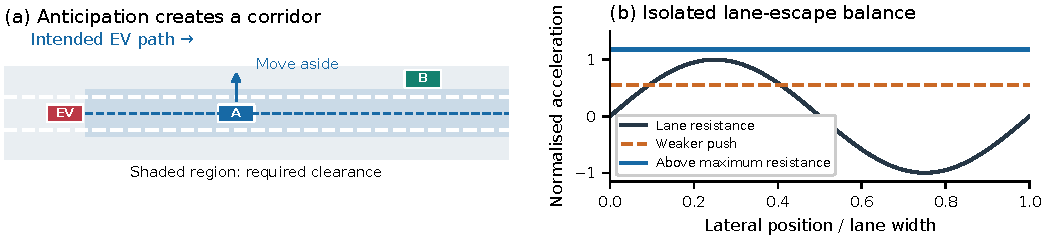
\includegraphics[width=0.915\textwidth]{model.pdf}
\caption{Conceptual mechanism. (a) Vehicle A still occupies the intended passage, whereas B has moved clear; the shaded region indicates required lateral clearance, not a prescribed trajectory. Geometry is schematic. (b) In the isolated constant-force approximation, a push above the maximum lane resistance removes the static lane-keeping equilibrium.}
\label{fig:model}
\end{figure*}

\section{Related Work}
SUMO represents emergency-vehicle behaviour through a native blue-light device and associated priority mechanisms~\cite{lopez18,bieker18}. These provide operational baselines; the present work emphasises explicit perception and continuous, parameterised responses of surrounding drivers.

Social force modelling~\cite{helbing95} and artificial potential fields for vehicle guidance~\cite{gerdes01,wolf08} motivate attractive and repulsive behavioural tendencies. A driving application additionally requires following-distance constraints, lane preference, bounded motion, and response timing. Cort\'es and Stefoni model EV interactions using observed emergency trips~\cite{cortes23}; Wu et al. optimise cooperative pre-clearing by connected vehicles~\cite{wu20}. Here the intended passage generates a continuous request whose execution depends on individual response and surrounding traffic.

Calibration must connect model structure to identifiable observables~\cite{punzo21,thiemann08}; ordinary lane changing also requires incentives and target-lane feasibility, as in MOBIL~\cite{kesting07}. The present formulation combines these requirements through shared lane-restoring dynamics and a predicted-corridor field, identifying host and emergency-response parameters separately.

\section{Model}
\label{sec:model}
\subsection{State, geometry, and behavioural accelerations}
Each vehicle $i$ carries position $(x_i,y_i)$, velocity $(v_{x,i},v_{y,i})$, dimensions $(L_i,W_i)$, desired speed $v_i^0$, driver parameters, awareness state, and urgency $u_i\in[0,1]$. The road is straight along $+x$; increasing $y$ points left. Lane $k$ has centre $(k+\tfrac12)w$, with lane zero rightmost and shoulders included in the drivable band. The implemented corridor projection is straight; curved-route prediction is outside the present formulation.

Specific forces are accelerations in m/s$^2$; longitudinal and lateral refer to motion along and across the road. We use $(z)_+=\max(z,0)$ and $\clip(z,a,b)=\min(\max(z,a),b)$. Figure~\ref{fig:model} introduces the intended passage and the competition between lateral push and lane resistance.



\subsection{Ordinary traffic and longitudinal composition}
The driving term relaxes the velocity toward the desired road-aligned motion:
\begin{equation}
\mathbf F_i^d=(v_i^0\hat{\mathbf x}-\mathbf v_i)/\tau_i.
\end{equation}
Thus $\tau_i$ controls the rate of speed recovery, while the lateral component damps sideways velocity. Neighbour repulsion uses floored bumper clearances $g_x,g_y$ and the elliptical metric
\begin{equation}
q_{ij}=\sqrt{(g_x/B_x)^2+(g_y/B_y)^2}.
\end{equation}
The magnitude $A_v e^{-q_{ij}}+A_n e^{-q_{ij}/q_n}$ combines ordinary and short-range repulsion. An outward elliptical direction and bearing weight $\lambda_v+(1-\lambda_v)(1+\cos\varphi_i)/2$ make nearby vehicles ahead more influential than those behind. The summed force is capped; repulsion discourages, but cannot preclude, overlap.

For each relevant leader, the intelligent-driver-model (IDM) interaction~\cite{treiber00} uses desired gap
\begin{equation}
s^*_{ij}=s_{0,i}+\pos{v_{x,i}T_i+
\frac{v_{x,i}\Delta v_{ij}}{2\sqrt{a_i b_i}}},
\end{equation}
where $s_{0,i}$ is standstill spacing, $T_i$ desired time headway, $a_i,b_i$ acceleration and comfortable-braking scales, and $\Delta v_{ij}$ closing speed. With bumper gap $s_{ij}$ and smooth lateral-overlap weight $o_{ij}$, the most restrictive leader gives
\begin{equation}
a_i^{I}=\min_j\left[-a_i\left(\frac{s^*_{ij}}{\max(s_{ij},0.3)}\right)^2o_{ij}\right].
\end{equation}
The longitudinal acceleration is composed as
\begin{equation}
a_{x,i}=F^d_{x,i}+\min(F^{cc}_{x,i}+F^E_{x,i}+F^c_{x,i},a_i^{I}).
\label{eq:compose}
\end{equation}
Here $F^{cc}$ is neighbour repulsion, $F^E$ the EV point field, and $F^c$ the corridor field. The minimum prevents the interaction component from relaxing the IDM demand; it also avoids adding every mild braking term to that demand. Subsequent acceleration limits and lateral motion remain relevant to safety.

\subsection{Perception and urgency}
An unaware compliant driver enters NOTICED when the EV is within an effective detection radius: 140 m for cars ahead of the EV nose and 60 m behind. A lognormal delay, with median 1 s and log-space standard deviation 0.45, precedes YIELDING. A sampled fraction $p_{nc}=0.05$ does not respond. These are effective perception assumptions.

At yield onset, an escape side $\sigma_i\in\{-1,+1\}$ is fixed for the episode. Vehicles clearly off the corridor line move farther to their own side; vehicles near it compare room to the road edges with a rightward bias. A driver enters HOLD after the EV passes by 8 m and is receding faster by more than 0.3 m/s. Following a 1.5--4 s recovery timer, ordinary awareness resumes. HOLD sets corridor urgency to zero while retaining point repulsion; it does not lock the vehicle at a fixed position.

Urgency represents response strength, distinct from the reaction delay. Define $S(z)=(1+e^{-z})^{-1}$, approach speed $v_a=\max(v_{x,E},0.6v_E^0)$, and
\begin{align}
t_i^{arr}&=s_i/\max(v_a-v_{x,i},0.5),\\
J_i&=\clip(1-v_{x,i}/15,0,1),\quad
T_i^{eff}=T_{react}(1+2.5J_i).
\end{align}
For vehicles ahead, $s_i$ is distance from the EV nose; behind it, arrival time is set to zero. The yielding-state urgency is
\begin{align}
u_i^{time}&=S((T_i^{eff}-t_i^{arr})/\sigma_t),\\
u_i^{prox}&=\max(J_i,g_p)S((R_u-s_i)/\sigma_s),\\
u_i&=\max(u_i^{time},u_i^{prox}).
\end{align}
The defaults are $T_{react}=9$ s, $\sigma_t=2.2$ s, $R_u=90$ m, $\sigma_s=12$ m, and proximity floor $g_p=0$. The factor $J_i$ grants slow traffic more anticipation; proximity urgency and the approach-speed floor prevent a blocked EV from removing its own clearing cue.

\subsection{Repulsion from the EV and its predicted corridor}
The EV point field acts on vehicles in YIELDING or HOLD:
\begin{align}
M_i^E&=\min(A_Ee^{(r_E-d_i)/B_E},F_{cap,E}),\\
\mathbf F_i^E&=G_iM_i^E
\left[\lambda_E+(1-\lambda_E)\frac{1+\cos\varphi_i}{2}\right]\hat{\mathbf n}_i.
\end{align}
$G_i$ is the awareness gate, $d_i$ the EV-to-car distance floored at 0.5 m, and $\hat{\mathbf n}_i$ the outward displacement divided by that distance. Bearing is measured against EV motion, with a forward fallback when nearly stopped. The default $\lambda_E=0.1$ favours forward response. This term is awareness-gated, rather than multiplied by urgency.

The corridor is anchored at the EV nose, centred on target line $y_c$, and extends $L_{back}=6$ m rearward and
\begin{equation}
L_c=\clip(\max(v_{x,E},0.6v_E^0)T_{pred},120,260)
\end{equation}
metres forward, with nominal $T_{pred}=8$ s. The minimum length retains an intended passage when the EV is blocked. Required centre clearance is $w_i^{need}=(W_E+W_i)/2+0.5$ m, and lateral offset is $d_{\perp,i}=y_i-y_c$. Let $f_i=\clip((L_c-s_i)/30,0,1)$ fade the final 30 m, and $g_i=u_if_i$ inside the longitudinal corridor and zero outside. Then
\begin{align}
F^c_{y,i}&=A_c e^{-\pos{|d_{\perp,i}|-w_i^{need}}/B_c}g_i\sigma_i,
\label{eq:corrlat}\\
F^c_{x,i}&=-\gamma_c g_i
\pos{1-|d_{\perp,i}|/w_i^{need}}\pos{v_{x,i}-\kappa v_i^0}.
\end{align}
The lateral request saturates within required clearance and decays outside it: $A_c$ sets strength and $B_c$ its lateral range. The longitudinal term slows a blocker toward $\kappa v_i^0$ to facilitate entry into adjacent gaps. Defaults are $\kappa=0.82$ and $\gamma_c=0.55$ s$^{-1}$.

\subsection{Lane keeping, escape, and numerical motion}
Lane preference is a periodic restoring force with effective amplitude
\begin{equation}
a_i^{eff}=a_{pin,i}(\rho_i/\rho_{ref})^{k_\rho}(1-\varepsilon u_i).
\label{eq:barrier}
\end{equation}
Density $\rho_i$ is measured in the vehicle's lane within $\pm100$ m, with $\rho_{ref}=10.61$ vehicles/km/lane. At fixed density and urgency, the potential and restoring term are
\begin{align}
U_i(y)&=-a_i^{eff}\frac{w}{2\pi}\cos\theta_i,\\
F^{pin}_{y,i}&=-a_i^{eff}\sin\theta_i,\quad
\theta_i=2\pi(y_i-y_i^{pref}-w/2)/w.
\end{align}
Its wells encode preferred lane positions, including personal offset $y_i^{pref}$. Urgency reduces resistance through $\varepsilon=0.5$; positive $k_\rho$ increases it with density. Exponential walls, supplementary damping, and hard road-edge projection complement lane keeping.

For an isolated vehicle under a constant push, no static lane equilibrium exists when $|F|>a_i^{eff}$: a \emph{depinning} condition. Inside an unfaded corridor, define $\chi_i=A_cu_i/a_i^{eff}$. Equating the decaying push to maximum restoring acceleration gives
\begin{equation}
d^*=w_i^{need}+B_c\ln\left(\frac{A_cu_if_i}{a_i^{eff}}\right),
\quad A_cu_if_i>a_i^{eff}.
\label{eq:dstar}
\end{equation}
This characteristic offset measures distance from the intended path to the car's centre, not a prescribed displacement or guaranteed corridor width. The logarithm follows by solving $A_cu_if_i\exp[-(d^*-w_i^{need})/B_c]=a_i^{eff}$. Below the escape threshold, linearising the restoring force gives within-lane displacement $\Delta y\approx Fw/(2\pi a_i^{eff})$: a driver can respond visibly without clearing the passage. For example, $w_i^{need}=2.5$ m, $B_c=2.8568$ m, and a push-to-resistance ratio of 1.68 give $d^*\approx3.98$ m. Neighbours, available road space, sinusoidal phase, and inertia determine actual settling.

Ordinary lane changes use comparative incentives: own frustration with a slower leader promotes overtaking, while pressure from a faster follower promotes moving right. A commitment requires an incentive above the effective threshold and an acceptable target-lane gap. A closing follower must leave time for both headway and lateral crossing. The lateral push is retained until the marking is crossed, or blocking or timeout cancels it. The fitted configuration shares lane resistance between ordinary and emergency manoeuvres; the optional separate commitment threshold is not used here.

Each step rebuilds the corridor, updates awareness and lane-change decisions, evaluates forces, and applies motion limits. Longitudinal composition follows \eqref{eq:compose}; lateral contributions are summed, then clipped. Semi-implicit Euler updates velocity before position, with nonnegative forward speed and bounded lateral speed. Nominal step is 0.05 s, with study-specific exceptions reported below. The automated EV uses a bounded lateral tracking spring instead of the periodic potential. These are road-frame kinematic constraints, not full steering or tyre dynamics.

\begin{figure*}[t]
\centering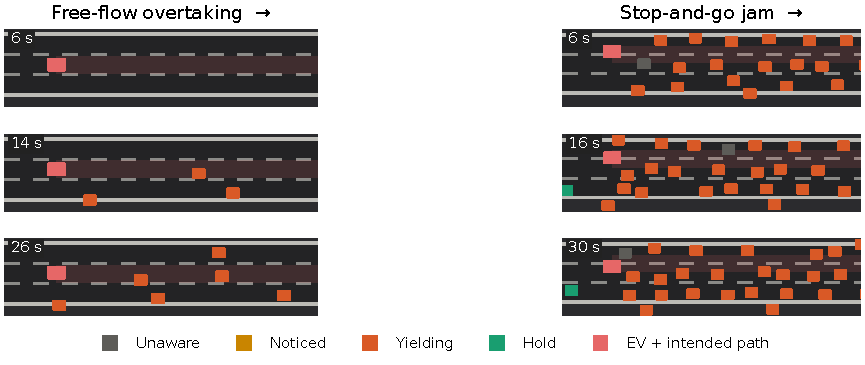
\includegraphics[width=0.915\textwidth]{snapshots.pdf}
\caption{Simulated corridor formation with the two-stage preset. Left: overtaking at 22 vehicles/km/lane, seed 1, at 6, 14 and 26 s. Right: stop-and-go jam, seed 3, at 6, 16 and 30 s. The view follows the EV; lateral scale is exaggerated twofold. The translucent strip marks the intended passage, rather than the vehicle-specific centre-clearance boundary.}
\label{fig:snapshots}
\end{figure*}

\section{Parameter Identification}
\label{sec:ident}
\subsection{Two-stage estimation and measurement consistency}
The shared restoring force links ordinary lane changing to emergency yielding. Fitting emergency manoeuvres alone can therefore confound a strong corridor request with weak lane discipline; an EV-free first stage constrains this ambiguity before the emergency block is estimated.
The earlier single-stage fit produced no discretionary lane changes in a recorded 206 vehicle-kilometre test without an active EV, despite the measured ordinary-traffic rate of about 0.28 per vehicle-kilometre. This motivates identifying the host dynamics before emergency response. Stage 1 uses highD~\cite{krajewski18}, comprising 60 German motorway drone recordings, approximately 110,000 vehicles and 44,000 vehicle-kilometres. Free-flow and dense regimes enter with equal weight; congested traffic is withheld.

The host block includes car following, lane keeping, driver heterogeneity, density dependence, and discretionary lane changing. Stage 2 freezes that block and estimates only $(A_E,B_E,A_c,B_c)$ from five processed EV-passage videos containing 144,896 vehicle observations. Perception timing, urgency, and longitudinal corridor braking remain fixed. The fitted EV amplitudes and ranges are $(5.9209,15.4181,2.3529,2.8568)$ in the corresponding acceleration and distance units.

Latin-hypercube screening and Nelder--Mead refinement use common random seeds~\cite{mckay79}. Matched detectors and observation windows ensure comparable lane-change statistics. Summary deviations are scaled, weighted, and capped; missing required observables receive the same ceiling of eight. The stage-1 objective combines summary and distribution-shape distances with overlap penalties, so suppressing lane changes cannot improve fit merely by making their duration undefined. Stage 2 compares kinematically labelled behavioural fingerprints, with additional TTC, overlap, and comfort penalties.

\subsection{Comparison levels and identification results}
An empirical reference should quantify variation in the data rather than be chosen to accommodate the fit. For ordinary traffic, each carriageway is compared with pooled summaries of the others. The mean leave-one-carriageway-out deviation across 88 free-flow carriageways is 0.49. It references the summary distance, not the full objective or safety.

The EV reference of 0.73 is computed differently: each video's fingerprint is compared with the pooled fingerprint including that video. It is therefore an inclusive-pool reference, not a strict leave-one-video-out estimate. EV validation uses fresh simulation seeds against the same recorded reference; this does not demonstrate transfer to unseen EV passages.

\begin{table}[t]
\caption{Identification outcomes. Lower scores indicate closer fit. Host rows report summary deviation; EV rows report the EV objective.}
\label{tab:ident}\centering\footnotesize
\setlength{\tabcolsep}{3.8pt}
\begin{tabular}{@{}lrrr@{}}\toprule
Evaluation & Two-stage & Earlier fit & Default\\\midrule
Host: fitted sites & 1.50 & 3.87 & 4.35\\
Host: held-out sites & 1.53 & 3.95 & 4.41\\
Host: dense regime & 0.84 & 3.33 & 3.80\\
Host: congested, held out & 2.48 & 3.81 & 3.51\\
\multicolumn{4}{@{}l}{Free-flow data reference: 0.49}\\\midrule
EV: fitting seeds & 0.94 & 1.27 & 1.13\\
EV: new seeds & 1.07 & 1.27 & 1.13\\
\multicolumn{4}{@{}l}{EV fingerprint reference: 0.73}\\\bottomrule
\end{tabular}
\end{table}

Table~\ref{tab:ident} shows that held-out host deviation decreases from 3.95 to 1.53, close to the fitted-site value of 1.50. This supports transfer of aggregate fit across sites, but 1.53 remains about 3.1 times the free-flow reference. In withheld congestion, 2.48 improves on the default 3.51 without establishing adequacy in that regime. The refitted EV block improves from 1.27 for the inherited EV settings to 0.94 on fitting seeds and 1.07 on new seeds. It too remains above its empirical reference. Improved fit and achieved adequacy must therefore be distinguished.

\section{Validation of the Formulation}
\label{sec:validation}
\subsection{Scenarios and observables}
Figure~\ref{fig:snapshots} shows simulated overtaking and stop-and-go scenarios using the two-stage preset. Time progresses downward; awareness colours distinguish response timing from completed movement. These are illustrative model realisations. The following tests examine internal mechanism consistency; the preceding trajectory comparison addresses empirical fit. Agreement in one does not establish the other.



EV progress is mean speed divided by desired speed. \emph{Forward clearance} is the bumper gap to the nearest vehicle blocking the required corridor, capped at 250 m and averaged over time. It differs from the \emph{lateral offset} used to test \eqref{eq:dstar}. Yield onset is the distance where YIELDING begins. Minimum time to collision (TTC) divides positive bumper gap by closing speed for relevant lateral footprints, assuming unchanged speeds.

The collision diagnostic counts overlapping pairs every second recorded frame, with a 0.05 m lateral tolerance. Persistent contact contributes repeatedly; \emph{overlap counts} therefore differ from distinct crashes and depend on recording cadence.

\subsection{Lane escape and characteristic lateral clearance}
The controlled escape sweep comprises $6\times3\times4=72$ combinations of $(A_c,B_c,a_{pin})$, three seeds per combination, with density modulation disabled. This sweep uses a 0.06 s integration step and 0.2 s requested recording interval. Eligible vehicles initially lie within required lateral clearance and enter a band 4--45 m ahead of the EV centre. The fraction $\phi$ has a settled offset beyond $w_i^{need}$, evaluated over the final 1.5 s in that band; $\phi_{onset}$ exceeds half that offset at any observed time.

\begin{figure*}[t]
\centering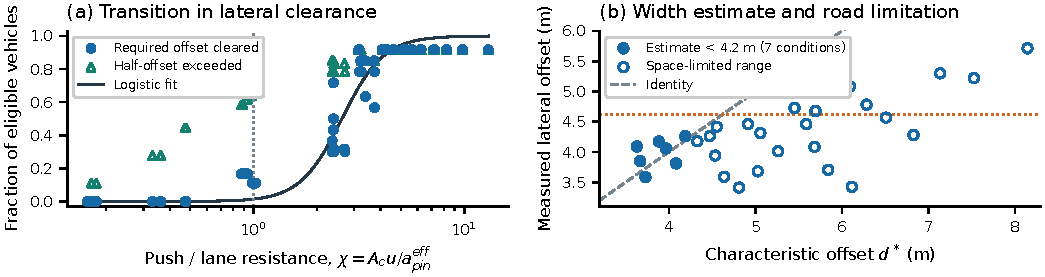
\includegraphics[width=0.915\textwidth]{depin.pdf}
\caption{Controlled tests of the force-balance interpretation. (a) Settled clearance and half-offset fractions against reduced push $\chi$; the logistic midpoint is 2.63. (b) Measured lateral offset versus \eqref{eq:dstar}, evaluated at measured urgency with $f=1$. Filled points identify the seven retained conditions below 4.2 m, with RMSE 0.25 m. The horizontal dotted line marks the reported saturation statistic near 4.6 m.}
\label{fig:depin}
\end{figure*}

Below $\chi=1$, mean settled-clearance fraction is 0.07, whereas the half-offset fraction is 0.41. The fitted settled-clearance curve has midpoint 2.63 and approaches saturation around $\chi=4$ (Fig.~\ref{fig:depin}a). This supports a transition in clearance but not an exact separator for complete lane changes. An isolated equilibrium criterion does not account for crowding, time-varying urgency, or finite manoeuvre duration.

For the width comparison, the statistic pools lateral offsets of yielding vehicles beyond required clearance in the same observation band, taking a median within each run and then across seeds. The reported analysis retains 30 conditions with finite estimates, pooled clearance fraction above 0.55, and $\chi>1.3$. Measured and estimated offsets have Spearman correlation 0.56. Within the seven retained conditions where $d^*<4.2$ m, root-mean-square deviation from identity is 0.25 m (Fig.~\ref{fig:depin}b). At larger estimates, the reported saturation statistic is approximately 4.6 m. Equation~\eqref{eq:dstar} is therefore useful within a restricted subset; it is not an unrestricted prediction of final position.

\subsection{The effect of anticipated path length}
The look-ahead experiment reduces the minimum corridor length to 10 m and varies $T_{pred}$ from 1 to 16 s at two free-flow densities, using five seeds. This isolates sensitivity to anticipation more directly than the nominal 120 m floor. At 22 vehicles/km/lane, shortening look-ahead from 8 to 1 s reduces speed ratio from 0.95 to 0.87, forward clearance from 65 to 47 m, and yield-onset distance from 92 to 61 m. Gains largely saturate by approximately 4 s (Fig.~\ref{fig:envelope}a). The 1 s case still contains a finite corridor; this is a short-anticipation comparison, not a point-field-only ablation.

\begin{figure*}[t]
\centering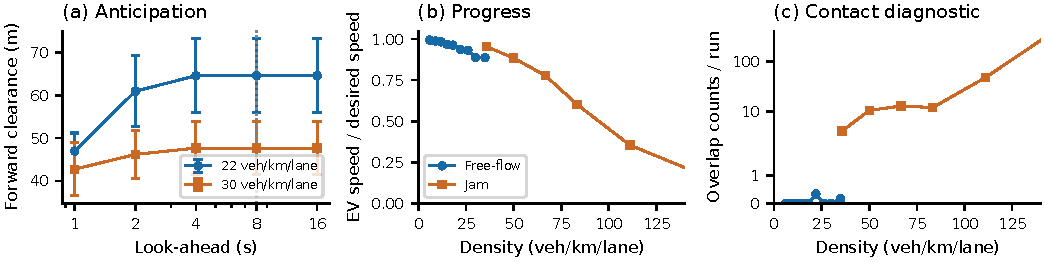
\includegraphics[width=0.915\textwidth]{envelope.pdf}
\caption{Anticipation and operating envelope. (a) Forward clearance versus look-ahead; error bars are one standard deviation across five seeds, with nominal 8 s marked. (b,c) Mean progress and overlap counts across six seeds. Jam density is the spacing-based equivalent $1000/\mathrm{spacing}$; it does not make jam geometry equivalent to free-flow traffic. The overlap axis is symmetric-logarithmic.}
\label{fig:envelope}
\end{figure*}

\section{Operating Envelope and Threats to Validity}
\label{sec:limits}
\subsection{Density, sensitivity, and numerical resolution}
Across the free-flow density sweep, EV speed ratio decreases from 0.99 at 6 to 0.89 at 35 vehicles/km/lane, and forward clearance decreases from 160 to 43 m. Mean overlap counts remain at or below approximately 0.3 per run, rather than identically zero. In the jam, overlaps occur at every tested spacing, increasing beyond 40 per run above an equivalent density of about 110 vehicles/km/lane; progress falls from 0.96 to 0.20 across the tested range. The lower-speed, tightly packed geometry lies outside the host calibration regime (Fig.~\ref{fig:envelope}b,c).

A one-at-a-time sweep of 29 parameters is complemented by a 180-sample joint Latin-hypercube screening~\cite{mckay79,saltelli08}. No single parameter changes free-flow speed ratio by more than 0.11 over its tested interval. In congestion, the largest one-at-a-time ranges arise from density exponent $k_\rho$ (0.72), lane strength $a_{pin}$ (0.59), urgency relief $\varepsilon$ (0.55), and non-response probability $p_{nc}$ (0.50). These are interval-dependent response ranges, not variance-based sensitivity indices. They identify lane resistance and response availability as priorities for congestion calibration.

\begin{table}[t]
\caption{Absolute relative change from the finest integration step, 0.0125 s. Maximum across free-flow and jam scenarios; rounded percentages.}
\label{tab:convergence}\centering\footnotesize
\begin{tabular}{@{}lrrrr@{}}\toprule
Step (s) & EV speed & Clearance & Min TTC & Onset\\\midrule
0.10 & 0.6\% & 0.6\% & 1.3\% & 0.3\%\\
\textbf{0.05} & 0.3\% & 0.1\% & 0.2\% & 0.5\%\\
0.025 & 0.1\% & 0.3\% & 0.1\% & 0.2\%\\\bottomrule
\end{tabular}
\end{table}

The time-step study compares 0.10, 0.05, 0.025, and 0.0125 s (Table~\ref{tab:convergence}). The four listed metrics at the nominal 0.05 s step differ by approximately 0.5\% or less from the finest step. This supports numerical robustness for these scenarios and observables; it does not establish collision-count convergence or stability throughout parameter space.

\subsection{Interpretation and simulator implications}
Three limitations constrain interpretation. First, the width statistic conditions on vehicles that moved aside, and its 0.25 m agreement concerns seven retained conditions. Second, EV recordings cover a limited set of passages; inclusive-pool comparison and new simulation seeds do not establish transfer to independent recordings. Third, the ordinary lane-change rate remains approximately 0.09 rather than the measured 0.28 per vehicle-kilometre. Sharing restoring strength between initiation and execution contributes to this tradeoff. Congestion and lane-change frequency remain unresolved even when individual manoeuvre statistics improve.

Integration changes control authority: the standalone model advances all vehicles; SUMO retains its dynamics under bounded field-derived requests; Unreal supplies human-driven EV kinematics while the force model advances surrounding traffic. These interfaces and their demonstration presets are not interchangeable. The current geometry is straight, detection is effective rather than acoustic, and lateral bounds do not constitute a complete vehicle-dynamics model. Neither the numerical studies nor the fit establishes training effectiveness; that requires evaluation with trainees.

\section{Conclusion}
The proposed model connects emergency-driver training needs to a causal sequence of perception, attempted yielding, constrained movement, and measurable corridor formation. Ordinary traffic supplies the lane preferences and interactions against which an EV's predicted-path request acts. An idealised lane-escape balance explains the principal control parameters, while controlled simulations delimit the accuracy of the characteristic-width estimate and demonstrate the value of anticipation. Two-stage identification improves held-out host fit and EV-response scores but does not reach the corresponding empirical references. The resulting framework is an interpretable basis for variable traffic responses, with congestion, independent passage validation, and trainee evaluation defining the next steps.

\balance
\begin{thebibliography}{10}\setlength{\itemsep}{0pt}\footnotesize

\bibitem{prohn20} M.~J. Prohn and B.~Herbig, ``Evaluating the effects of a
simulator-based training on knowledge, attitudes and driving profiles of German
ambulance drivers,'' \emph{Accid. Anal. Prev.}, vol.~138, art.~105466, 2020.

\bibitem{custalow04} C.~B. Custalow and C.~S. Gravitz, ``Emergency medical
vehicle collisions and potential for preventive intervention,'' \emph{Prehosp.
Emerg. Care}, vol.~8, no.~2, pp.~175--184, 2004.

\bibitem{lopez18} P.~A. Lopez \emph{et al.}, ``Microscopic traffic simulation
using SUMO,'' in \emph{Proc.\ IEEE ITSC}, 2018, pp.~2575--2582.

\bibitem{bieker18} L.~Bieker-Walz, M.~Behrisch, and M.~Junghans, ``Analysis of
the traffic behavior of emergency vehicles in a microscopic traffic
simulation,'' \emph{EPiC Series in Engineering}, vol.~2, pp.~1--13, 2018.

\bibitem{helbing95} D.~Helbing and P.~Moln\'ar, ``Social force model for
pedestrian dynamics,'' \emph{Phys. Rev. E}, vol.~51, no.~5, pp.~4282--4286, 1995.

\bibitem{gerdes01} J.~C. Gerdes and E.~J. Rossetter, ``A unified approach to
driver assistance systems based on artificial potential fields,'' \emph{J. Dyn.
Syst. Meas. Control}, vol.~123, no.~3, pp.~431--438, 2001.

\bibitem{wolf08} M.~T. Wolf and J.~W. Burdick, ``Artificial potential functions
for highway driving with collision avoidance,'' in \emph{Proc. IEEE ICRA}, 2008,
pp.~3731--3736.

\bibitem{cortes23} C.~E. Cort\'es and B.~Stefoni, ``Trajectory simulation of
emergency vehicles and interactions with surrounding traffic,'' \emph{J. Adv.
Transp.}, vol.~2023, art.~5995950, 2023.

\bibitem{wu20} J.~Wu, B.~Kulcs\'ar, S.~Ahn, and X.~Qu, ``Emergency vehicle lane
pre-clearing: From microscopic cooperation to routing decision making,''
\emph{Transp. Res. Part B}, vol.~141, pp.~223--239, 2020.

\bibitem{treiber00} M.~Treiber, A.~Hennecke, and D.~Helbing, ``Congested traffic
states in empirical observations and microscopic simulations,'' \emph{Phys. Rev.
E}, vol.~62, no.~2, pp.~1805--1824, 2000.

\bibitem{kesting07} A.~Kesting, M.~Treiber, and D.~Helbing, ``General
lane-changing model MOBIL for car-following models,'' \emph{Transp. Res. Rec.},
vol.~1999, pp.~86--94, 2007.

\bibitem{punzo21} V.~Punzo, Z.~Zheng, and M.~Montanino, ``About calibration of
car-following dynamics of automated and human-driven vehicles,'' \emph{Transp.
Res. Part C}, vol.~128, art.~103165, 2021.

\bibitem{thiemann08} C.~Thiemann, M.~Treiber, and A.~Kesting, ``Estimating
acceleration and lane-changing dynamics from next generation simulation
trajectory data,'' \emph{Transp. Res. Rec.}, vol.~2088, pp.~90--101, 2008.

\bibitem{krajewski18} R.~Krajewski, J.~Bock, L.~Kloeker, and L.~Eckstein, ``The
highD dataset: A drone dataset of naturalistic vehicle trajectories on German
highways for validation of highly automated driving systems,'' in \emph{Proc.
IEEE ITSC}, 2018, pp.~2118--2125.

\bibitem{mckay79} M.~D. McKay, R.~J. Beckman, and W.~J. Conover, ``A comparison
of three methods for selecting values of input variables in the analysis of
output from a computer code,'' \emph{Technometrics}, vol.~21, no.~2,
pp.~239--245, 1979.

\bibitem{saltelli08} A.~Saltelli \emph{et al.}, \emph{Global Sensitivity
Analysis: The Primer}. Chichester, U.K.: Wiley, 2008.

\end{thebibliography}

\end{document}
